\documentclass[a4paper]{jpconf}
% \bibliographystyle{iopart-num}
\usepackage{amsmath}
\usepackage{citesort}
\usepackage{subfigure}
\usepackage{graphicx}
\graphicspath{{fig/}}
\usepackage{ifpdf}
\ifpdf\usepackage{epstopdf}\fi
\usepackage[export]{adjustbox}

%----------------------------------------------------- 
%\usepackage{soul,ulem,color,xspace,bm}
% Suggest to remove
%\newcommand{\asrm}[1]{{\color{magenta}\sout{#1}}}
% Suggest to insert
%\newcommand{\as}[1]{\color{cyan}#1\xspace\color{black}}
% Suggest to replace
%\newcommand{\asrp}[2]{\asrm{#1} \as{#2}}
% Comment
%\newcommand{\ascm}[1]{{\color{green}\;AS: #1}}
%------------------------------------------------------

\def\apj{ApJ}
\def\mnras{MNRAS}
\def\nat{Nat}
\def\prd{Phys. Rev. D}
\def\araa{ARA\&A}                % "Ann. Rev. Astron. Astrophys."
\def\aap{A\&A}                   % "Astron. Astrophys."
\def\aaps{A\&AS}                 % "Astron. Astrophys. Suppl. Ser."
\def\aj{AJ}                      % "Astron. J."
\def\apjs{ApJS}                  % "Astrophys. J. Suppl. Ser."
\def\pasp{PASP}                  % "Publ. Astron. Soc. Pac."
\def\apjl{ApJ}                   % letter at ApJ
\def\pasj{PASJ}
\def\apss{Astroph. Space Sci.}
\def\aplett{Astroph. Lett}
\def\ssr{Space Sci. Rev.}
\def\aapr{Astron. Astroph. Reviews}
\def\physrep{Phys. Reports}
\def\memsai{Mem. Societa Astronom. Italiana}
\def\jgr{JGR}
\def\jcap{Journal of Cosmology and Astroparticle Physics}

\usepackage{xspace}
\usepackage[dvipsnames]{xcolor}
\usepackage[normalem]{ulem}
% Suggest to remove
\newcommand{\asrm}[1]{{\color{OrangeRed}\sout{#1}}}
% Suggest to insert
\newcommand{\as}[1]{\color{RoyalBlue}#1\xspace\color{black}}
% Suggest to replace
\newcommand{\asrp}[2]{\asrm{#1} \as{#2}}
% Comment
\newcommand{\ascm}[1]{{\color{ForestGreen}#1}}

\begin{document}
	\title{PIC simulation of instabilities in relativistic supernovae shocks}
	
	\author{V I Romansky$^{1}$, A M Bykov$^{1,2}$ and S M Osipov$^{1}$}
	
	\address{$^1$ Ioffe Institute, 26 Politekhnicheskaya st., St. Petersburg 194021, Russia}
	\address{$^2$ Peter the Great St. Petersburg Polytechnic University, 29 Politekhnicheskaya st., St. Petersburg 195251, Russia}
	
	\ead{romanskyvadim@gmail.com}
	
	\begin{abstract}
                 Modern observations show presence of relativistic supernovae - objects intermediate between regular supernovae and gamma-ray bursts. The typical lorentz-factors of plasma flows in relativistic supernovae are about $1.5$. The process of cosmic ray acceleration is very different from both non-relativistic and ultra-relativistic case. In this paper is presented particle-in-cell modeling of trans-relativistic collisionless shocks. It is shown, that development of magneto-hydrodynamic instabilities, particularly Bell's instability, has strong influence on cosmic ray acceleration. At times larger than $1500$ reverse ion plasma frequency magnetic field, generated by Bell's instability, significantly suppresses the electrons spectrum. This effect should be taken into account for modeling of synchrothron spectrum from relativistic supernovae.
	\end{abstract}
	
	\section{Introduction}
	Relativistic jets and winds are the generic outflows of the relativistic supernovae \cite{2010Natur.463..513S,2007ApJ...667..351W}, the accreting black holes, both suprmassive in the active galactic nucleis  \cite{1984RvMP...56..255B} as well as the stellar masses in the gamma-ray burst sources, microquasars \cite{2019MmSAI..90...57M,1999PhR...314..575P,2014LNP...876.....R} and pulsar wind nebulae \cite{2019MNRAS.488.5690O,2017SSRv..207..235B,2017JPlPh..83e6301K,2019ApJ...876L...8B}. Relativistic shocks can be formed either inside the flow of low or moderate magnetization (the internal shocks) or can be driven by the outflow colliding with the ambient medium (the external shocks). In many cases the relatistivistic shocks in astrophysical objects are collisionless and are often associated with non-equilibrium particle distributions \cite{2012SSRv..173..309B,2015SSRv..191..519S,2017SSRv..207..319P}. They can accelerate particles to ultra-high energies \cite{2009JCAP...11..009L}. On the one hand, the presence of non-maxwellian components with very long equilibration time requires a kinetic description of the shocked flows. The kinetic structure of relativistic shocks can be modelled within the particle-in-cell approach, which allows one to properly account for the electron scale processes and for the density of the displacement current which is important in relativistic plasma flows.  On the other hand, available computer capabilities do not alow one to provide a fully kinetic modelling of the macroscopic astrophysical flows and, therefore, the fluid MHD description based on such macroscopic parameters as the effective adiabatic index of the flow is widely used. Here we discuss an approach allowing to determine the effective adiabatic indexes from the microscopical particle-in-cell modeling of the mildly-relativistic shocks typical for the relativistic supernovae and gamma-ray burst afterglows.   
	
	
	\section{Numerical setup}
	In this work we use particle-in-cell code Smilei \cite{Smilei18} for modeling trans-relativistic collisionless shocks. We initialize two-dimensional space domain, with electron-proton plasma flowing into simulation box through the right boundary and reflecting wall on the left boundary. In the transversal direction boundary conditions are periodic.
	
	The simulation parameters are : the initial flow Lorentz factor $\Gamma = 1.5$, the flow magnetization $\sigma = \frac{B^2}{4\pi\Gamma (n_p m_p + n_e m_e) c^2} = 0.004$. The dimensionless thermal energy $\Delta \gamma = \frac{k T}{m_p c^2}$ is equal to $10^{-4}$ and the electron mass is increased up to $m_e = \frac{m_p}{100}$. The size of the simulation box along the $x$ axis is $L_x = 30000\frac{c}{\omega_p}$ and in the transverse direction $L_y = 200\frac{c}{\omega_p}$, where $\omega_p = \sqrt{\frac{4\pi q^2 n}{\Gamma m_e}}$ is the plasma frequency. These scales correspond to $150000$ and $1000$ grid points in $x$ and $y$ directions, respectively. 
	
	Inclination angle of magnetic field due to shock velocity is $\theta = 30$ degrees, which corresponds to the maximum efficiency of particle acceleration \cite{Romansky18} and magnetic field is lying in the simulation plane.
	
	
	\section{Results}
	
	Profiles of transversal magnetic field, obtained from numerical simulation, show significant field amplification in precursor of shock wave, see figure \ref{field}. It is result of development of instabilities in plasma, particularly Bell instability \cite{Bell04}, which grows rate is larger then grows rate of other instabilities.
	
	\begin{figure}[h!]
		\centering
		\includegraphics[width=0.8\textwidth]{fig/Bnorm.png} 
		\caption{Evolution of the magnetic field in time.}
		\label{field}
	\end{figure}
	
	Spectrum of electrons is shown in figure \ref{spectrum}. One can see, that electrons distribution function at high energies $(\gamma > 300)$ is maximal at times about 1500 inverse protons plasma frequencies and at the longer times spectrum decreases. It may by explained as consequence of magnetic field amplification. Instabilities increase the transverse magnetic field and also the angle between field and shock velocity. As a result shock becomes superluminal \cite{Sironi2011} and can not effectively accelerate particles.
	
	
	\begin{figure}[h!]
		\centering
		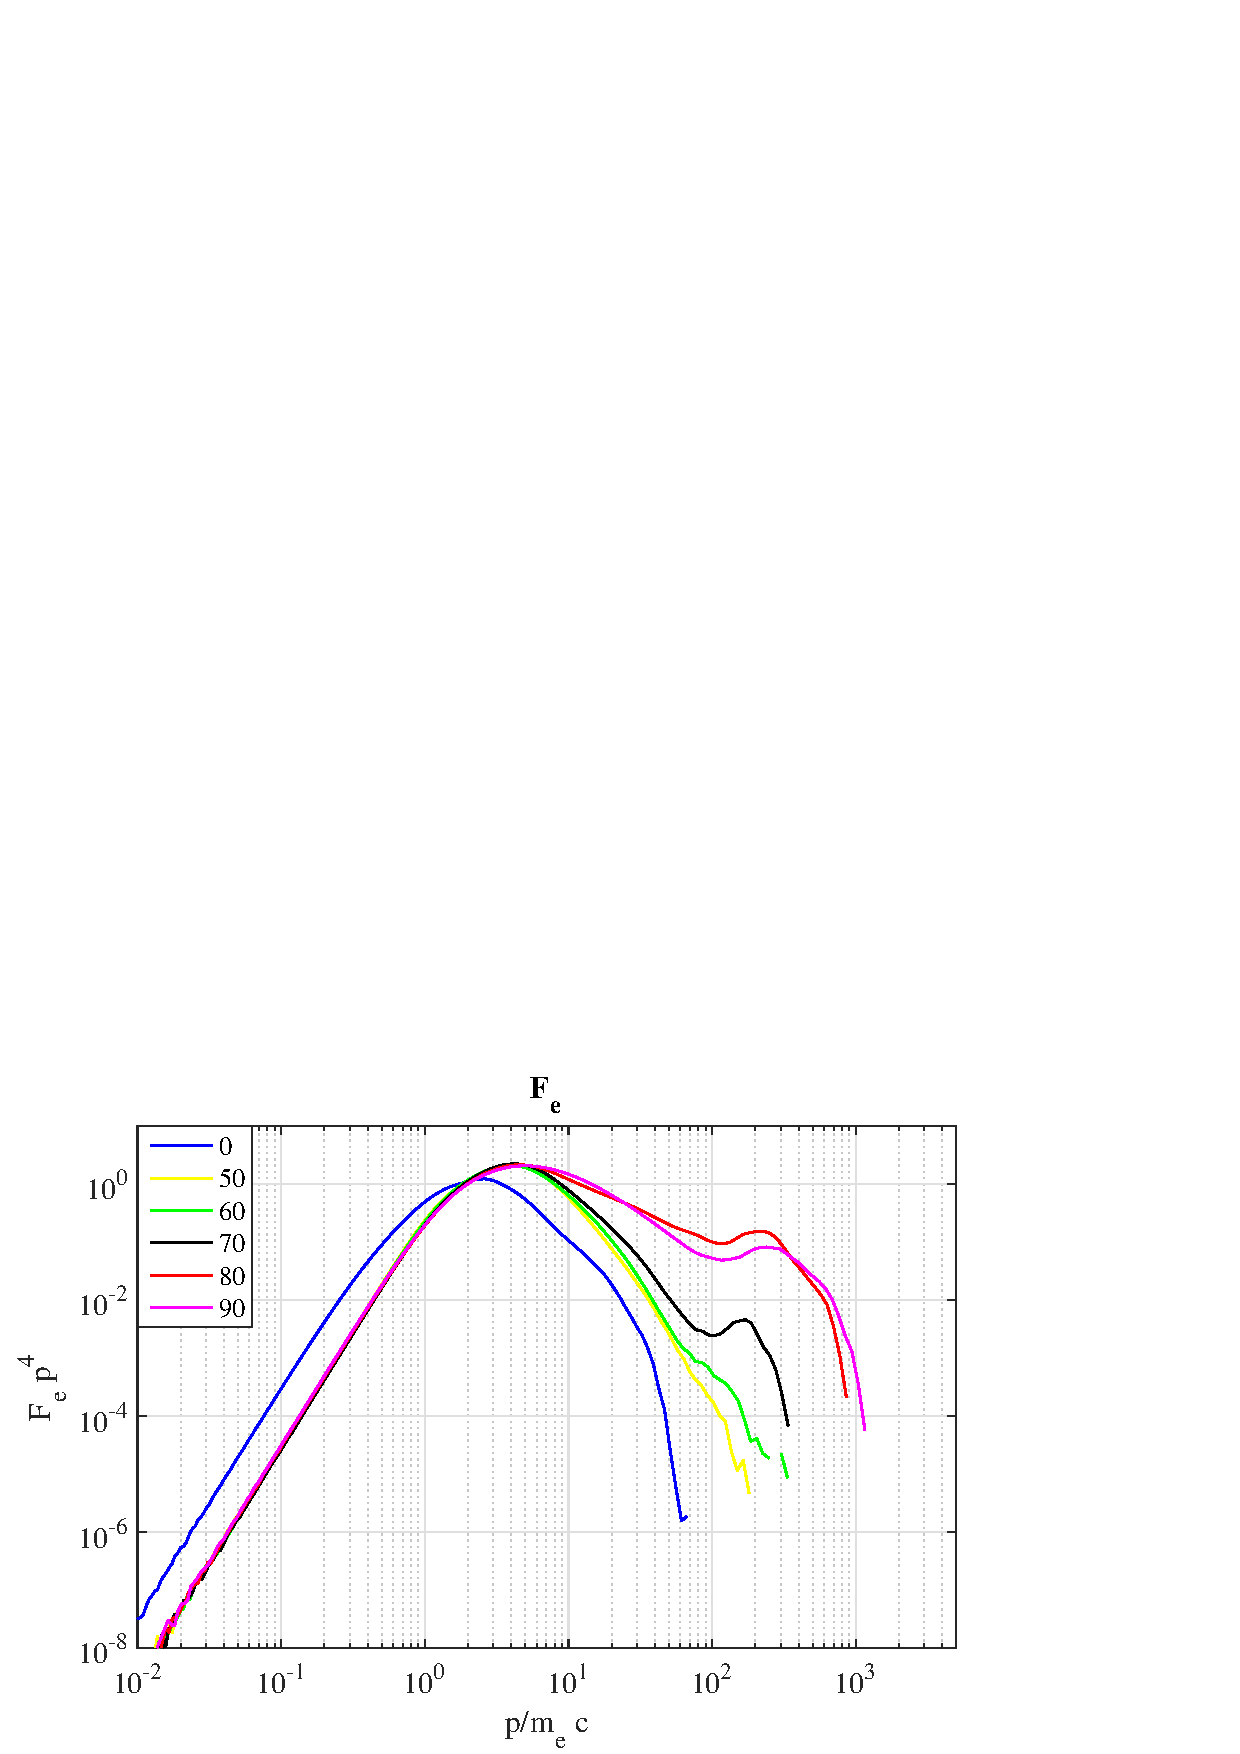
\includegraphics[width=0.8\textwidth]{fig/spectrum.png} 
		\caption{Evolution of the electrons spectrum in time.}
		\label{spectrum}
	\end{figure}
	

	
	\section{Conclusions}
	
	Particle-in-cell simulations have been used to derive effective macroscopic parameters of relativistic shocks in space plasmas. The effective adiabatic index and electron temperatures are two important parameters required to supplement large-scale single-fluid magneto-hydrodynamic simulations of processes in astrophysical plasmas. The adiabatic indexes for the downstream flow derived with PiC method are summarized in Table 1 and can be used for MHD modeling of relativistic
	supernovae. Further modelling is needed to study the dependence of these two parameters on the initial conditions which, reflect the presence of MHD large-scale turbulence in the stellar wind of the progenitor massive star upstream of the  mildly-relativistic shock of the supernova. 
	
	\ack
	V I Romansky and A M Bykov acknowledge a support from RSF grant 16-12-10225.
	Results of the work were obtained using computational resources of Peter the Great Saint-Petersburg Polytechnic University Supercomputing Center (http://scc.spbstu.ru)
	
	\section*{References}
	% \bibliographystyle{apalike}
	\bibliographystyle{iopart-num}

	\bibliography{bibliogr}
\end{document}